% !TeX root = RJwrapper.tex
\title{Navigating the R Package Universe}
\author{by Julia Silge, John C. Nash, Spencer Graves}

\maketitle

\abstract{%
Today, the enormous number of contributed packages available to R users
outstrips any given user's ability to understand how these packages
work, their relative merits, or how they are related to each other. We
organized a plenary session at useR!2017 in Brussels for the R community
to think through these issues and ways forward. This session considered
three key points of discussion. Users can navigate the universe of R
packages with (1) capabilities for directly searching for R packages,
(2) guidance for which packages to use, e.g., from CRAN Task Views and
other sources, and (3) access to common interfaces for alternative
approaches to essentially the same problem.\\
}


\hypertarget{introduction}{%
\section{Introduction}\label{introduction}}

As of our writing, there are over 13,000 packages on CRAN. R users must
approach this abundance of packages with effective strategies to find
what they need and choose which packages to invest time in learning how
to use. At \href{https://user2017.brussels/}{useR!2017 in Brussels}, we
organized a plenary session on this issue, with three themes:
\textbf{search}, \textbf{guidance}, and \textbf{unification}. Here, we
summarize these important themes, the discussion in our community both
at useR!2017 and in the intervening months, and where we can go from
here.

Users need options to search R packages, perhaps the content of
DESCRIPTION files, documentation files, or other components of R
packages. One author (SG) has worked on the issue of searching for R
functions from within R itself in the \CRANpkg{sos} package \citep{sos}.
Other options have been built such as
\href{https://www.rdocumentation.org/}{RDocumentation.org}
\citep{rdocumentation}.

Guidance about what package to use for any given task is available from
multiple resources for users. R users can turn to long-established
resources like \href{https://cloud.r-project.org/web/views/}{CRAN Task
Views} \citep{ctvs}, or newer options under current development such as
\pkg{packagemetrics} \citep{packagemetrics} or the
\CRANpkg{CRANsearcher} RStudio addin \citep{cransearcher}. One author
(JS) organized a survey before useR about how R users learn about R
packages that informed our discussion and is summarized here.

By unification, we largely mean meta-packages or wrappers, packages that
call other, related packages for a common set of tasks. A unified
wrapper package provides a common
\href{https://en.wikipedia.org/wiki/Application_programming_interface}{API}
through which to access many different implementations for a certain
task. One author (JN) has been particularly involved in numerical
optimization techniques and presented possibilities there and beyond.
More generally, as revealed during breakout discussions at useR!2017 and
beyond, there are opportunities to merge either packages or their
functionality. Such ideas require human cooperation and some give and
take in a realm where egos can take precedence over ease of use.

After our main presentation at useR!2017, we broke out into three
smaller sessions focused on these themes. We are encouraged by the
engaged attendance and vigorous participation from the community we
experienced, and hope to use our community's enthusiasm and ideas to
move forward with steps that will improve the value of the R ecosystem
to humanity.

\hypertarget{search}{%
\section{Search}\label{search}}

There are a number of different search capabilities for R, with
different characteristics and strengths. The ways to search for help
using R have proliferated in much the same way that the number of
packages has, with some of the same challenges. It is not clear to users
what the best way to search is, and many if not most users are not even
aware of the search capabilities that have been built.

The R Project for Statistical Computing's website has had a page focused
on \href{https://www.r-project.org/help.html}{``Getting Help with R''}
\citep{gettinghelp} from early in R's history. This official overview of
various help facilities recognized by the R Core Team includes functions
such as \code{help()}, \code{demo()}, \code{apropos()},
\code{help.search()}, and vignettes. This search and help functionality,
used from R itself, accesses only locally installed documentation. This
page also currently points to resources such as the CRAN Task Views, FAQ
pages, Stack Overflow, and R email lists.

Other search capabilities have been developed by the R community over
the years, focused on different types of searching. The
\href{http://search.r-project.org/nmz.html}{R Site Search} built by
\citet{baron} is one of the longest running, and can also be accessed
from R itself using the \texttt{RSiteSearch()} function in
\CRANpkg{utils} \citep{utils} and the \CRANpkg{sos} package. The
\code{sos::findFn()} function returns a \code{data.frame} of class
\code{findFn} summarizing the help pages matching a search term. These
objects can be combined by union and intersection, summarized by
package, and output to an Excel file with sheets giving one row for each
package and for each help page sorted by package.

The \href{https://rseek.org}{rseek} site of \citet{goodman} is another
resource that has been available for over a decade, and searches not
only documentation but also GitHub issues, social media, and more. The
\href{https://rdrr.io}{R Package Documentation} site of \citet{rdrrio}
is a newer option that includes not only a way to search R documentation
but also the ability to run R in the browser. Another full-featured and
modern website for search is
\href{https://www.rdocumentation.org/}{RDocumentation.org}, which offers
users the ability to contribute examples.

Other options for search capability focus not on documentation or
individual functions but on packages and package descriptions. The
search capability at \href{https://www.r-pkg.org/}{METACRAN}
\citep{metacran}, \href{http://www.crantastic.org/}{crantastic}
\citep{crantastic}, and the RStudio addin \CRANpkg{CRANsearcher} allow
users to search the descriptions and titles of packages to find tools
that fit their analysis needs.

This discussion of search options for R users is intended to be thorough
but not entirely exhaustive, and to demonstrate the variety of resources
available. Many search sites are not clear how to use their search
capabilities (single words vs.~structured queries), and the algorithms
used for ranking results give disparate results. An additional point to
be considered is to what extent these options for search are open
source, and what affect that could have, either positive or negative.
For example, the source code for both METACRAN and
\CRANpkg{CRANsearcher} is entirely open on GitHub while
RDocumentation.org is maintained by DataCamp, a privately held company.

The analysis in this section is summarized in a
\href{https://en.wikiversity.org/wiki/Searching_R_Packages}{Wikiversity
article} \citep{wikiversity}; the article is on Wikiversity so anyone
can contribute to it. At useR!2017, after the large contributed session,
we broke out into three smaller sessions for discussion and
brainstorming. In the breakout session focused on search, some
participants commented that user reviews, available on at least
\href{http://www.crantastic.org/}{crantastic} among these existing
resources, are useful alongside search. The discussion overall led to
the development of a draft proposal for improving the ability of R users
to search R packages, which is available on Wikiversity; anyone can
contribute to moving it closer to realization \citep{draftProposal}.
Overall, perhaps it is time for the R Project for Statistical
Computing's \href{https://www.r-project.org/search.html}{``Search''}
\citep{search} page to include more updated options.

\hypertarget{guidance}{%
\section{Guidance}\label{guidance}}

In preparation for this session, one author (JS) ran a brief online
survey in the spring of 2017 to ask R users how they currently discover
and learn about R packages. The results of this survey are available in
an R package \pkg{packagesurvey} \citep{packagesurvey} on GitHub. There
were 1039 respondents to this survey, which had a single multiple select
question on it, ``How do you currently discover and learn about R
packages?''

\begin{Schunk}
\begin{table}

\caption{\label{tab:unnamed-chunk-2}Percentage of respondents who chose each answer on survey}
\centering
\begin{tabular}[t]{ll}
\toprule
How do you currently discover and learn about R packages? & \% of respondents\\
\midrule
Social media such as blogs, R-bloggers, Twitter, Slack, or GitHub contacts & 79.8\%\\
General search websites such as Google and Yahoo & 57.0\%\\
Your personal network, such as colleagues and professors & 41.6\%\\
Books, textbooks, or journal articles (JSS, JOSS, R-Journal) & 31.9\%\\
Conferences, meet-ups, or seminars & 24.1\%\\
\addlinespace
CRAN Task Views & 21.8\%\\
Email lists such as r-help, r-packages, or r-pkg-devel & 15.3\%\\
R-specific search websites such as METACRAN or Rdocumentation & 11.1\%\\
Other & 4.2\%\\
R packages built for search such as the sos package & 2.2\%\\
\bottomrule
\end{tabular}
\end{table}

\end{Schunk}

Responses to this survey were fielded from R email help lists, local R
meetup groups, social media such as Twitter, and affinity groups such as
R-Ladies. Figure 1 shows when users responded to the survey. The
respondents to this survey overwhelmingly look to social media including
blogs and Twitter to learn about R packages, and also make use of
general search sites and their personal network.

There were helpful, insightful answers from people contributing to the
``other'' option. R users use Stack Overflow to learn about R packages,
as well as options like
\href{http://dirk.eddelbuettel.com/cranberries/}{CRANberries}
\citep{cranberries} and \href{http://www.crantastic.org/}{crantastic},
both of which have RSS feeds that users follow. Other users mentioned
learning by reading code on GitHub, the R Special Interest Group mailing
lists \citep{mailinglists} such as \texttt{r-sig-mixed-models} and
\texttt{r-sig-geo}, and other search websites including
\href{http://rpackages.io/}{rpackages.io}.

\begin{figure}
  \centering
  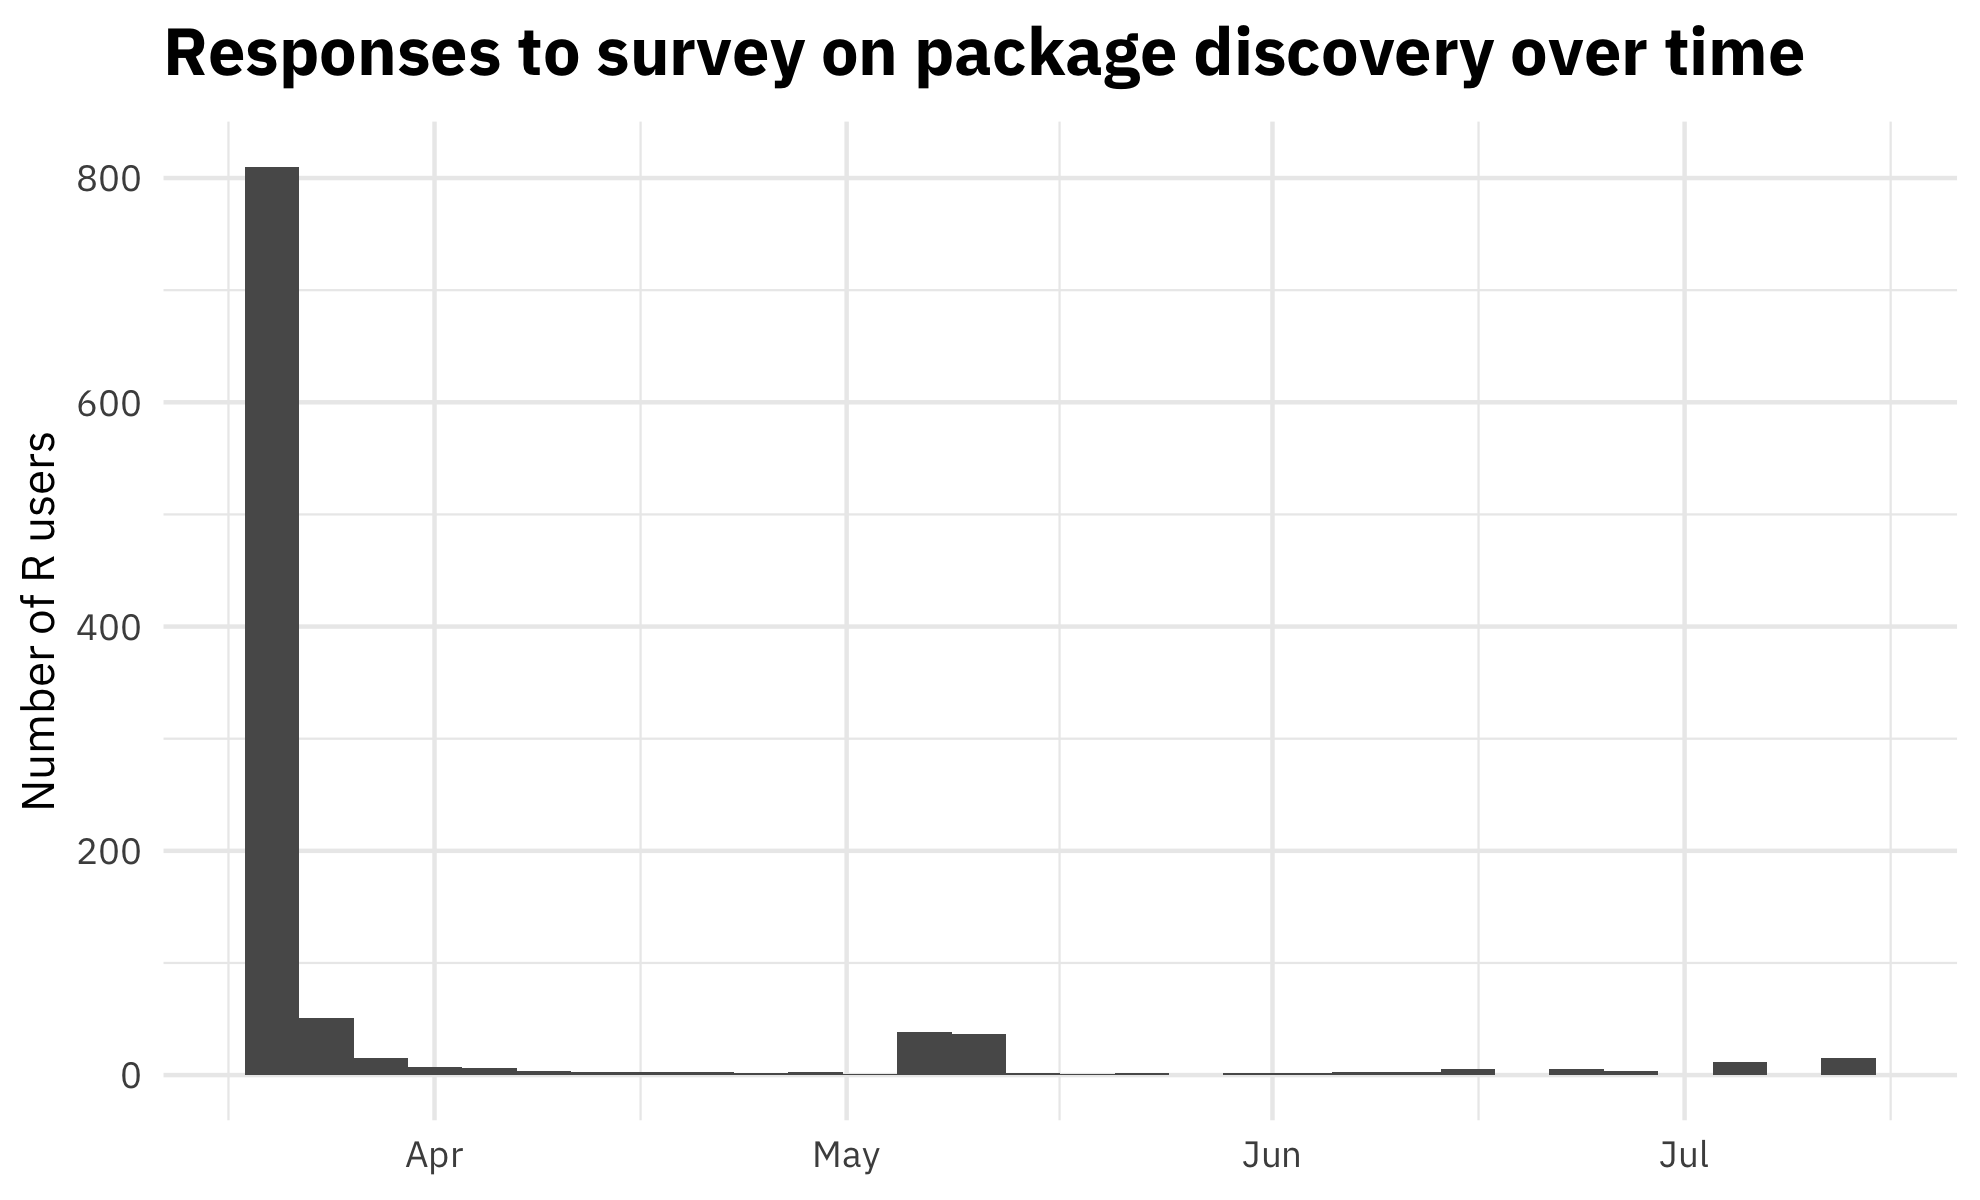
\includegraphics[scale=0.2]{survey_time-1}
  \caption{Responses to survey on package discovery during the spring of 2017}
  \label{figure:survey_time}
\end{figure}

In the breakout session at useR!2017 focused on guidance for package
choice and package evaluation, we had about 40 participants in our
discussion. It was a fruitful discussion and several important themes
emerged.

\hypertarget{value-of-personal-impact}{%
\subsection{Value of personal impact}\label{value-of-personal-impact}}

Participants in this session emphasized how impactful personal
relationships can be in how packages are shared and evaluated. Some
participants discussed how building local networks of R users may be
more important in this effort than top-down, technological solutions.
Our survey does show that personal recommendations have been important
for many individuals in evaluating R packages. This is yet another area
where local user groups can continue to have important impact. Some ways
to share this experience more broadly would be online video series or
live data analysis, such as those by
\href{https://www.facebook.com/seanjtaylor/videos/10103088186201897/}{Sean
Taylor} \citep{taylor} and \href{https://youtu.be/jWePleDwmQo}{Roger
Peng} \citep{peng}. Learning through personal networks does not
invalidate the importance of other tools like search, especially when it
comes to more specialized tasks.

\hypertarget{cran-task-views}{%
\subsection{CRAN Task Views}\label{cran-task-views}}

Some participants wondered whether the idea of a CRAN Task View
\citep{ctvs} is outdated in the current climate with so many packages,
and whether it is even possible for one person to maintain one
effectively. In fact, several participants voiced frustration with CTVs
that have focused on older packages alone. Others responded that CTVs
are focused on curation, which \emph{is} still important, perhaps even
more so now in a world with over 13,000 packages. We had at least one
CTV maintainer present in our breakout session, and several things were
presented as important in order for CTV maintainers to do their jobs:

\begin{itemize}
\tightlist
\item
  Package maintainers should update their \texttt{NEWS} files.
\item
  Package maintainers need to write good documentation.
\end{itemize}

These are helpful for \emph{all} R users, of course, but also for
maintainers of CRAN Task Views. The \CRANpkg{pkgdown} \citep{pkgdown}
package was mentioned as an effective option to make documentation
visible.

\hypertarget{cran-and-you}{%
\subsection{\texorpdfstring{CRAN and
\emph{you}}{CRAN and you}}\label{cran-and-you}}

Participants had several ideas about how things are done on CRAN now and
adjustments that might be made in the interest of discovering and
evaluating packages. One idea that came up several times was the
possibility of keywords or tagging for packages. Since useR!2017, the
authors have learned that there is support for some tagging architecture
for packages on CRAN in the
\href{https://cran.r-project.org/doc/manuals/r-release/R-exts.html\#The-DESCRIPTION-file}{DESCRIPTION
file using ACM, JEL, or MSC classifications}. For an example of this in
action, check out the \CRANpkg{lfe} \citep{lfe} package. These are
fairly unwieldy lists currently and something like an RStudio addin
could be used to navigate them, if they were widely used.

Another desire participants voiced was for more information directly on
CRAN, such as the number of downloads for packages. Participants also
suggested that vignettes for context-specific tasks like the
\href{https://www.bioconductor.org/packages/release/workflows/}{Bioconductor
Workflows} \citep{bioc} would be helpful for package discovery and
evaluation, either associated with CRAN or perhaps the \emph{R Journal}.
Finally, there was some discussion about whether gate-keeping on CRAN,
perceived by most to be reasonable and minimal currently, is good or bad
for the community. The conclusion in our discussion was that increased
editorial efforts to keep packages off CRAN would not be positive for
our community.

\hypertarget{more-data-more-problems}{%
\subsection{More data, more problems}\label{more-data-more-problems}}

Some of the package developers at the session wondered why, when R is a
data-centric language, developers have such primitive analytics about
their users. Issues of user privacy are central here, but there might be
opt-in options that could help both package developers and users make
better decisions. The idea of a recommender system for R packages was
brought up multiple times, perhaps a Tinder for R packages like
\href{https://simplystatistics.org/2016/10/03/papr/}{papr, the Tinder
for academic preprints} \citep{papr}. Both the users and developers
present thought that data on package use (instead of package downloads
alone) would be helpful in evaluating how important or helpful R
packages are. Participants also discussed the possibility of a linter
for analysis scripts, similar in concept to linters for code (such as
\citet{lintr}) that automatically analyze code for potential problems
and errors, that would suggest packages and good practice. Such a linter
would necessarily be opinionated, but almost all efforts to suggest and
evaluate R packages are, by definition.

\hypertarget{unification}{%
\section{Unification}\label{unification}}

\textbf{Unification}, as we describe it here, attempts to reduce the
package count and the span of knowledge required of users. When there
are many ways to carry out the same calculation, there are inevitable
differences of approach. However, in many respects it is the
\textbf{similarity} of approaches that causes most confusion. Very
similar calling sequences, unless they are entirely compatible, lead to
confusing experiences for users, and threaten the validity of results.

From the experience of one author (JN), the most satisfactory form of
unification from the user perspective is the use of wrapper functions
that consolidate a number of similar tools into a single calling
sequence. This has been the goal of the package \CRANpkg{optimx}, which
in its 2018 incarnation consolidates several R-internal and
package-based function minimization tools. Moreover, the present version
subsumes a number of other packages, thereby offering a reduction in the
effective package count.

A real downside of unification is the burden of work for the developers
involved, including dealing with complex dependencies \emph{and} reverse
dependencies. At the time of writing, the new \CRANpkg{optimx} fails
reverse dependency checks because of new, stricter checks for CRAN
policies. Embracing unification as an approach to deal with package
proliferation means that such issues are a part of life and must be
resolved.

While a wrapper such as \CRANpkg{optimx} can, with effort, be created,
merging two existing but different packages that provide similar
capability with very different user interfaces requires human
cooperation. At this time, and despite the open and collaborative R
community, the level of effort to do such work is daunting. Moreover,
there is a general lack of financial or other reward for such efforts.

During discussions at useR!2017, it was clear that R users are quite
interested in unification of packages. Younger participants expressed
the opinion that there are egos and interest groups standing in the way
of some such unifications, and the status of some of the players impeded
the discussion of such possibilities.

\hypertarget{conclusion}{%
\section{Conclusion}\label{conclusion}}

Our exploration of these topics leads us to call for increased respect
and value for the work done by local meetup group organizers and
individuals who contribute to spreading R knowledge, both online and in
their communities. Our survey and discussions show how impactful these
community networks are; investing in community building is not something
we need do only because of idealism, but because it is effective.

We also see the importance of continued commitment to growing the skills
of package developers across the R ecosystem. Adopting best practices,
including understanding dependency management and writing good
documentation, makes this entire challenge better for everyone, from the
developer with downstream dependencies to the CRAN Task View maintainer
to the new R user.

\bibliography{RJreferences}


\address{%
Julia Silge\\
Stack Overflow\\
110 William Street, Floor 28\\ New York City, NY 10038\\
}
\href{mailto:julia.silge@gmail.com}{\nolinkurl{julia.silge@gmail.com}}

\address{%
John C. Nash\\
University of Ottawa\\
Telfer School of Management\\ Ottawa, ON K1N 6N5, Canada\\
}
\href{mailto:nashjc@uottawa.ca}{\nolinkurl{nashjc@uottawa.ca}}

\address{%
Spencer Graves\\
EffectiveDefense.org\\
4550 Warwick Blvd. Apt. 508\\ Kansas City, MO 64111\\
}
\href{mailto:spencer.graves@effectivedefense.org}{\nolinkurl{spencer.graves@effectivedefense.org}}

